
\usetikzlibrary{arrows.meta,calc}

\begin{frame}{simple network model}
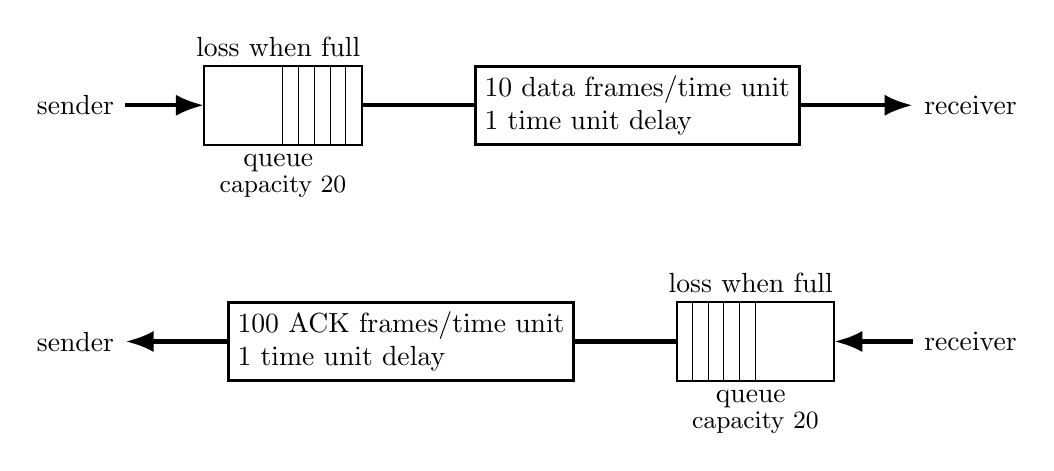
\begin{tikzpicture}
\draw[ultra thick,arrows={-Latex}] (0, 0) node[left] {sender} -- (1, 0);
\draw[thick] (1, -.5) rectangle (3, .5);
\foreach \x in {2,2.2,2.4,2.6,2.8} {
    \draw (\x, -.5) -- (\x, .5);
}
\node[anchor=south,align=center] at (2, .5) {
    loss when full
};
\node[anchor=north,align=center] at (2, -.5) (queue label) {
    queue
};
\node[anchor=north,font=\small] at ([yshift=.2cm]queue label.south) {
    capacity 20
};
\draw[ultra thick,arrows={-Latex}] (3, 0) -- (10, 0) node[right]{receiver}
    node[midway,fill=white,draw=black,very thick,align=left] {
        10 data frames/time unit \\
        1 time unit delay
    };
\begin{scope}[shift={(10, -3)},x=-1cm]
    \draw[ultra thick,arrows={-Latex}] (0, 0) node[right] {receiver} -- (1, 0);
    \draw[thick] (1, -.5) rectangle (3, .5);
    \foreach \x in {2,2.2,2.4,2.6,2.8} {
        \draw (\x, -.5) -- (\x, .5);
    }
    \node[anchor=south,align=center] at (2, .5) {
        loss when full
    };
    \node[anchor=north,align=center] at (2, -.5) (queue label) {
        queue
    };
    \node[anchor=north,font=\small] at ([yshift=.2cm]queue label.south) {
        capacity 20
    };
    \draw[ultra thick,arrows={-Latex}] (3, 0) -- (10, 0) node[left]{sender}
        node[midway,fill=white,draw=black,very thick,align=left] {
            100 ACK frames/time unit \\
            1 time unit delay
        };
\end{scope}
\end{tikzpicture}
\begin{itemize}
\item simulator from upcoming assignment
    \begin{itemize}
    \item command line \texttt{--delay 1 --bandwidth-forward 10 --bandwidth-backward 100 --buffer 30}
    \end{itemize}
\end{itemize}
\end{frame}

\begin{frame}{exercise: forward latency}
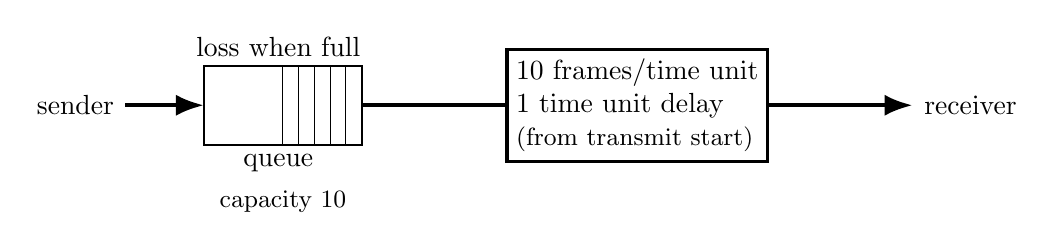
\begin{tikzpicture}
\draw[ultra thick,arrows={-Latex}] (0, 0) node[left] {sender} -- (1, 0);
\draw[thick] (1, -.5) rectangle (3, .5);
\foreach \x in {2,2.2,2.4,2.6,2.8} {
    \draw (\x, -.5) -- (\x, .5);
}
\node[anchor=south,align=center] at (2, .5) {
    loss when full
};
\node[anchor=north,align=center] at (2, -.5) (queue label) {
    queue
};
\node[anchor=north,font=\small] at (queue label.south) {
    capacity 10
};
\draw[ultra thick,arrows={-Latex}] (3, 0) -- (10, 0) node[right]{receiver}
    node[midway,fill=white,draw=black,very thick,align=left] {
        10 frames/time unit \\
        1 time unit delay \\
        \small (from transmit start)
    };
\end{tikzpicture}
\begin{itemize}
\item minimum latency = 1 time unit
\item exercise: maximum latency?
\end{itemize}
\begin{tabular}{lll}
A. 1 time unit & B. 1.1 time unit & C. 1.2 time unit \\
C. 1.4 time unit & D. 1.9 time unit & E. 2.0 time unit \\
F. 2.1 time unit & G. something else \\
\end{tabular}
\end{frame}
